\section{関連研究} \label{sec:RelatedResearch}

多カテゴリにおけるレーティング予測に関する従来研究、
及び、提案手法に関連した研究、技術について述べる。
はじめに提案手法で用いているパラグラフベクトルと深層学習について述べる。
次に、レーティング予測について、多カテゴリのものを対象とした従来手法と
ニューラルネットワークを用いた手法について述べる。
最後に、その他本研究で利用した技術について述べる。


\subsection{パラグラフベクトル}

パラグラフベクトルは、文や文書といった大きな単位の言語表現の意味表現を
学習する手法である。
これは、Continuous BOW (CBOW)またはSkip-gram\cite{yoshua03}という
単語の意味表現の学習手法を応用した手法である。
ここではCBOWを応用したDistributed Memory model of Paragraph Vectors (PV-DM)
について説明する。
PV-DMはBOWと異なり、単語の並び順を考慮した文や文書の分散表現を
生成することができる。

\begin{figure}
  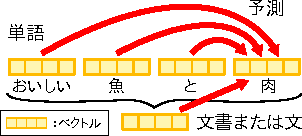
\includegraphics[0.5]{fig/paragraph_vector_v2.pdf}
  \caption{パラグラフベクトルの学習の概略}
  \label{fig:ParagraphVector}
\end{figure}

以下に具体的なアルゴリズムを示す。
ここでは文書の意味表現を学習する場合について考える。
学習の概略を図\ref{fig:ParagraphVector}に示す。
まず、意味表現を学習する対象となる文書に含まれる単語を
初めから一つずつ読んでいく。
その際、現在の単語及びその周辺の単語、現在の文書について、
式\ref{eq:ParagraphVector}に示す目的関数$L$を最大化するように
各パラメータの学習を行う。
\begin{gather} \label{eq:ParagraphVector}
  L = \sum_d L_d \\
  L_d = \frac{1}{T} \sum^{T}_{t = k} \log p(w_t | w_{t-k}, ..., w_{t-1}),
     \nonumber \\
  p(w_t | w_{t-k}, ..., w_{t-1}) = \frac{e^{y_{w_t}}}{\sum_i e^{y_i}},
    \nonumber \\
  y = b + Uh(w_{t-k}, ..., w_{t-1}, d; W, D) \nonumber
\end{gather}
ここで、$L_d$は文書$d$の目的関数である。
$w_i$は単語、$W$は全ての単語の分散表現を表す行列、
$D$は全ての文書の分散表現を表す行列である。
$k$はウィンドウサイズ、$T$は現在の文書に含まれる単語数である。
ある単語の周辺を表す区間をウィンドウという。
$p$はsoftmax関数により正規化された、文脈から現在の単語が導かれることの
尤度である。
$p$を構成する$y$は現在の単語とウィンドウ内の単語及び現在の文書から導出される。
$h(w_{t-k}, ..., w_{t-1}, d; W, D)$は引数となるベクトルを平均したベクトル
または結合したベクトルを返す関数である。

PV-DMによって生成したレビューの文書のベクトルを
ニューラルネットワークによって分類することで、
レーティング予測においてBOW等より高い正答率が得られることが示されている。
しかし、文書全体にパラグラフベクトルを用いる場合、文同士の位置関係が
予測時に考慮できない。


\subsection{深層学習}

深層学習とは、多層のニューラルネットワークを用いた
機械学習の手法の総称である\cite{takayuki15}。
以下には、その内ニューラルネットワークの正則化を行うための2つの手法、
ドロップアウトと重み減衰について述べる。
また、提案手法と直接関係がないが、関連するニューラルネットワークによる
レーティング予測の手法\cite{nal14,rie14,duyu15}で用いられているため、
畳み込みニューラルネットワークについても説明する。

ドロップアウトとは、ニューラルネットワークにおける層のニューロンの数を
一時的に減らすことによって正則化を行う方法である。
ある層に対してドロップアウトを行うには、その層が持つニューロンの出力値を
確率的に0とする。
%また、出力値が0となったニューロンに対する重みの勾配は0となるため、
%そのニューロンに対する重みはその学習回において更新されない。
これを各学習回で行うことで、ニューラルネットワーク全体を学習する。

次に、重み減衰について説明する。
重み減衰とは、ニューラルネットワークの各重みをその大きさに応じて
学習回毎に減少させる正則化の手法である。
重み減衰を行うためには、ニューラルネットワークの最小化すべき目的関数に対して
各重みの2ノルムを足し合わせる。
式\ref{eq:NNObjectiveWithWeightDecay}に、重み減衰を適用した目的関数$L'$示す。
\begin{gather} \label{eq:NNObjectiveWithWeightDecay}
  L' = L + \frac{\lambda}{2} \sum_{\mathbf{w}} {|\mathbf{w}|}^2
\end{gather}
ここで、$L$はニューラルネットワークの重み減衰を適用していない目的関数である。
$\mathbf{w}$はニューラルネットワークの各層における重みである。
$\lambda$は重みの減衰率である。
式\ref{eq:NNObjectiveWithWeightDecay}により、
ニューラルネットワークのある層の重み$\mathbf{w}$に対する
更新式は式\ref{eq:WeightUpdateEquation}のようになる。
\begin{gather} \label{eq:WeightUpdateEquation}
  \mathbf{w} \leftarrow \mathbf{w} - \frac{\partial L}{\partial \mathbf{w}}
                                   - \lambda \mathbf{w}
\end{gather}
ここで、$a \leftarrow b$は変数$a$の値をそのときの式$b$の値で
更新することを示す。
ただし、全結合層のバイアス等では一般に重み減衰を行わない。
これはそのような重みの値は場合によって大きい値を取る必要があるためである。

最後に、畳み込みニューラルネットワークについて説明する。
畳み込みニューラルネットワークとは、畳み込み層とプーリング層を用いた
ニューラルネットワークである。
一般に、畳み込み層とプーリング層は交互に配置される。
畳み込みニューラルネットワークは入力の局所的な特徴を抽出することができる。
また、畳み込みニューラルネットワークは元々画像認識に応用されていた手法であり、
その入力は複数のチャネルを持つことがある。
チャネルとは、画像でいうRGBの各色のことである。
例として、畳み込みニューラルネットワークの入力をRGB画像とした場合、
それは(チャネル)×(画像の幅)×(画像の高さ)の3次元行列で表される。
以下では、複数チャネルを持つ画像に対して畳み込みニューラルネットワークを
適用する場合の畳み込み層とプーリング層について説明する。

畳み込み層とは、前の層の各ニューロンが
それと位置の近い次の層のニューロンとしか結合しないように
全結合層を単純化した層である。
具体的にはある$H \times H$の大きさを持つフィルタを考え、
それを畳み込み層の入力値に適用して値を出力する。
図\ref{fig:ConvolutionalLayer}にその概略を示す。
\begin{figure}
  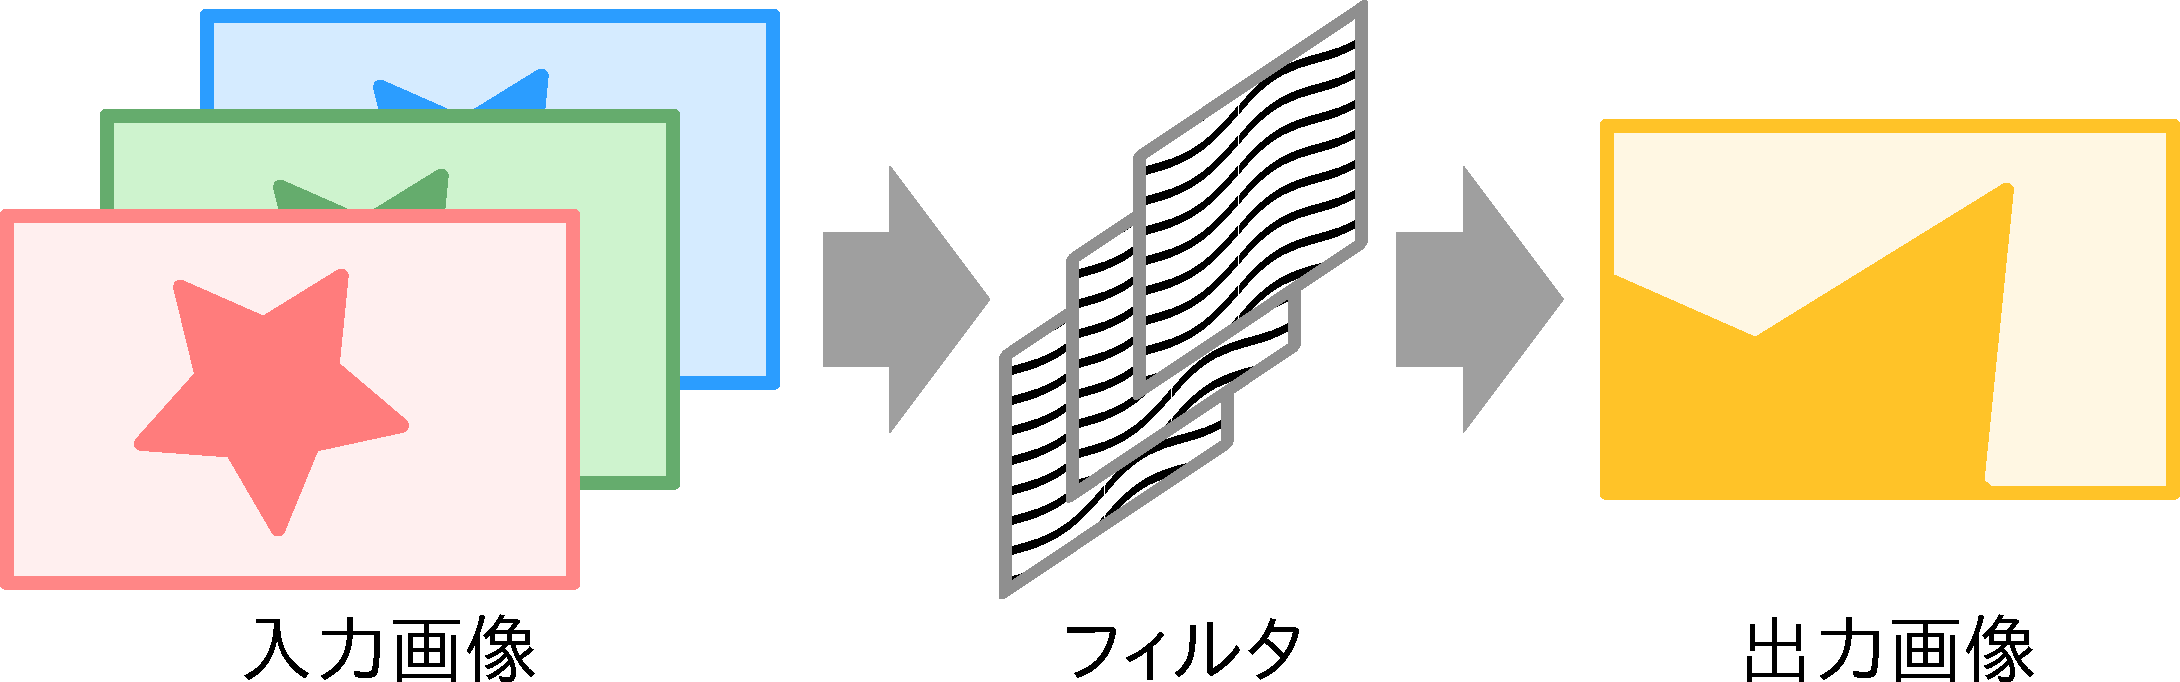
\includegraphics[0.7]{fig/convolutional_layer_with_one_filter.pdf}
  \caption{畳み込み層の概略}
  \label{fig:ConvolutionalLayer}
\end{figure}
式\ref{eq:ConvolutionalLayerFilter}に、畳み込み層のフィルタ$f$によって
処理された出力値$u_{fij}$を示す。
\begin{gather} \label{eq:ConvolutionalLayerFilter}
  u_{fij} = \sum^{C - 1}_{c = 0} \sum^{H - 1}_{p = 0} \sum^{H - 1}_{q = 0}
            z^{(l - 1)}_{c, i + p, j + q} h_{fcpq} + b_{fij}
\end{gather}
ここで、$z^{(l - 1)}_{c, i + p, j + q}$は、前の層$l - 1$の出力値である。
$H$はフィルタの幅である。
$h_{fcpq}$はチャネル$c$に対するフィルタ$f$の重みである。
$b_{fij}$はフィルタ$f$のバイアスである。
ただし、バイアスの値は位置によらず一つのフィルタ内で共有することが多い。
$(i, j)$は出力画像における位置である。
$(p, q)$はフィルタ$f$における位置である。
最終的な畳み込み層の出力値$z_{fij}$は$u_{fij}$の値に活性化関数を適用し
計算する。
\begin{gather} \label{eq:ConvolutionalLayerOutput}
  z_{fij} = \sigma(u_{fij})
\end{gather}
ここで、$\sigma$は活性化関数である。
実際の畳み込み層は複数のフィルタを持つことが多い。

次に、プーリング層とは入力画像の局所的な平均や最大値を取る層である。
これによって、入力画像における特徴の位置に関するノイズを緩衝できる。
式\ref{eq:PoolingLayer}に、平均プーリング層の出力値の位置$(i, j)$における
出力値$u_{cij}$を示す。
\begin{gather} \label{eq:PoolingLayer}
  u_{cij} = \frac{1}{H^2} \sum_{(p, q) \in P_{ij}} z_{cpq}
\end{gather}
ここで、$H$はプーリングする範囲の幅である。
$P_{ij}$は出力画像の位置によるプーリングの範囲であり、位置の集合で表される。
$c$はチャネルである。
$(i, j)$は出力画像における位置である。
$(p, q)$はあるプーリングの範囲$P_{ij}$における入力画像での位置である。


\subsection{レーティング予測}

商品レビューにおけるレーティング予測とは、レビューの文書から
そのレビューに対して実際にユーザが付与したレーティングを予測する問題である。
ここではレーティング予測に関する研究の内、まず本研究の従来研究である
藤谷ら\cite{fujitani15}の研究について説明する。
その後、深層学習を用いたレーティング予測手法について説明する。

\subsubsection{隠れ状態を用いたホテルレビューのレーティング予測}

藤谷ら\cite{fujitani15}は複数のカテゴリにおけるレーティング予測に対して、
Multi-Instance Multi-Label learning for Relation Extraction (MIML-RE)
\cite{mihai12}モデルを用いた手法を提案している。
その手法では、レビュー内の各文毎に予測した隠れレーティングから
レビュー全体のレーティングを予測する。
図\ref{fig:FujitaniRelationsAmongRatingCategories}のように、
文毎のレーティングからレビュー全体のレーティングを予測する際の
カテゴリ間の繋がりを手動で変化させカテゴリ間の関係性を考慮している。
各文の素性にはBag Of Words (BOW)またはBag Of n-gramsを用いている。
藤谷ら\cite{fujitani15}は各文毎に隠れレーティングを予測することによって
0.4832の正答率が得られることを示した。
また、カテゴリ間の繋がりによって正答率が変化することを示した。

\begin{figure}
  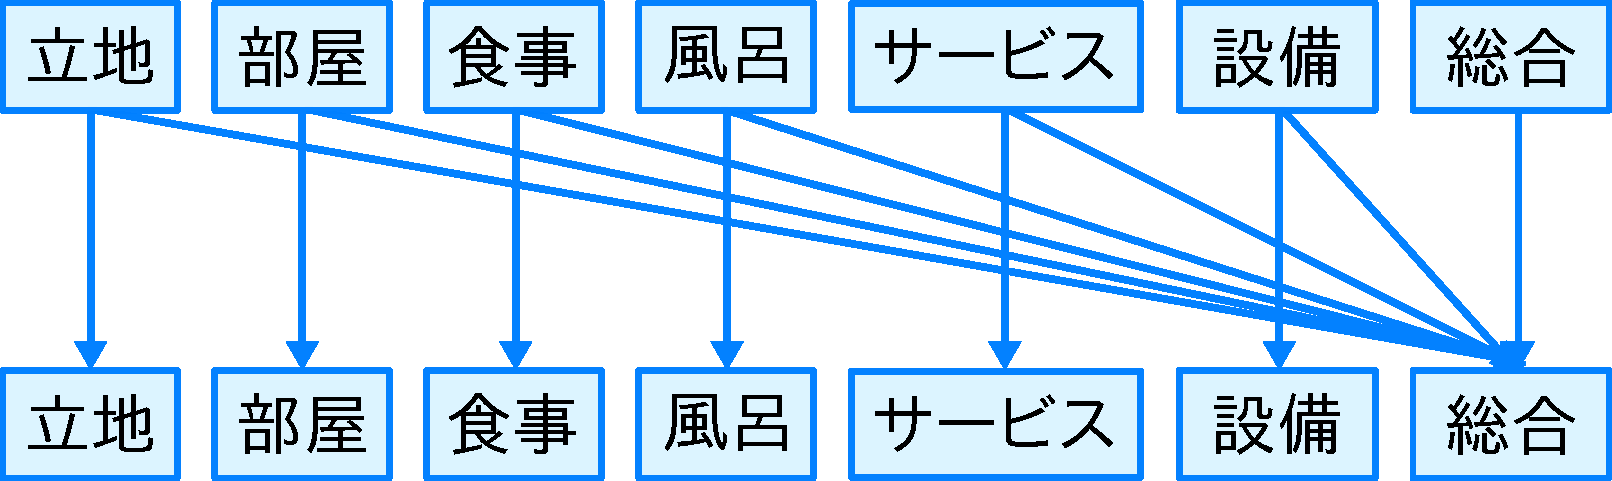
\includegraphics[0.5]
      {fig/fujitani_miml_relations_among_rating_categories.pdf}
  \caption{藤谷ら\cite{fujitani15}のモデルにおけるカテゴリ同士の繋ぎ方の例}
  \label{fig:FujitaniRelationsAmongRatingCategories}
\end{figure}

この手法では、文同士の位置関係を考慮しておらず、
カテゴリ間については考慮しているものの複雑な関係を捉えることができていない。

\subsubsection{深層学習を用いたレーティング予測}

深層学習を用いたレーティング予測の手法が、Nalら\cite{nal14}、
Rieら\cite{rie14}、Duyuら\cite{duyu15}等によって提案されている。
これらの方法に共通するのは、単語や文の意味表現から
畳み込み\nn と全結合\nn を用いて予測を行うことである。
これらの手法では、まず、畳み込み層によって入力の局所的な素性を捉える。
その後、畳み込み\nn から得られた文書全体の素性を
全結合\nn の入力とし多値または二値分類を行う。
また、Duyuら\cite{duyu15}とNalら\cite{nal14}の手法は
\nn のモデルの中にパラメータとして単語の意味表現を取り込んでいる。
これにより、特定の分類問題に対してそれらを最適化することができる。

Nalら\cite{nal14}は、単語の素性から文の素性を表現する、
分類や生成に適したモデルを提案している。
このモデルはDynamic Convolutional Neural Network (DCNN)と呼ばれる。
DCNNは畳み込み層とdynamic k-max pooling層、folding層、全結合層を
を組み合わせた多層の\nn である。
DCNNの畳み込み層はMax - Time Delay Neural Network (Max-TDNN)\cite{ronan08}
という文の意味を表現する\nn のモデルに基づいている。
Max-TDNNは、単語ベクトルの各次元毎に1次元フィルタを持った畳込み層と
その出力値に対して次元毎に最大値プーリングを行う層の2層と全結合層から
構成される\nn である。
dynamic k-max pooling層は、プーリングの範囲からk個の最大値を
その順序を保持したまま取り出す層である。
このとき、$l$番目の畳み込み層の後のプーリングにおける$k$の値、$k_l$は
式\ref{KOfDynamicKMaxPooling}によって計算される。
\begin{gather} \label{KOfDynamicKMaxPooling}
  k_l = \max ( k_{top}, \lceil \frac{L - l}{L}s \rceil )
\end{gather}
ここで、$top$は最後の畳み込み層であり、
$L$はDCNNに含まれる畳み込み層の総数である。
$s$は入力文に含まれる単語の総数である。
また、folding層は入力となる行列を列方向に2行ずつ足し合わせる層である。
レーティング予測の実験において、Support Vector Machine (SVM)や
他の\nn を用いた手法と比較して、DCNNは高い正答率を示した。

Rieら\cite{rie14}はseq-Convolutional Neural Network (seq-CNN)と
bow-Convolutional Neural Network (bow-CNN)の2つの手法を提案している。
seq-CNNとbow-CNNの共通点は、文書の素性から畳み込み\nn と全結合\nn によって
レーティング予測を行うことである。
相違点は文書の素性である。
seq-CNNにおける文書の素性は、(語彙の大きさ)×(領域の大きさ)だけの
次元を持つベクトルからなる行列である。
図\ref{fig:SeqCNNTextFeature}のように、
文書はある単語数の領域毎に一定の単語数ずつずらしながら
分割され、行列に変換される。
ここで、領域とはある単語数を持つ文書内の区間のことである。
語彙の大きさだけの次元を持つベクトルは1つの単語を表すone-hotベクトルである。
(語彙の大きさ)×(領域の大きさ)だけの次元を持つベクトルは
それらを結合したベクトルである。
\begin{figure}
  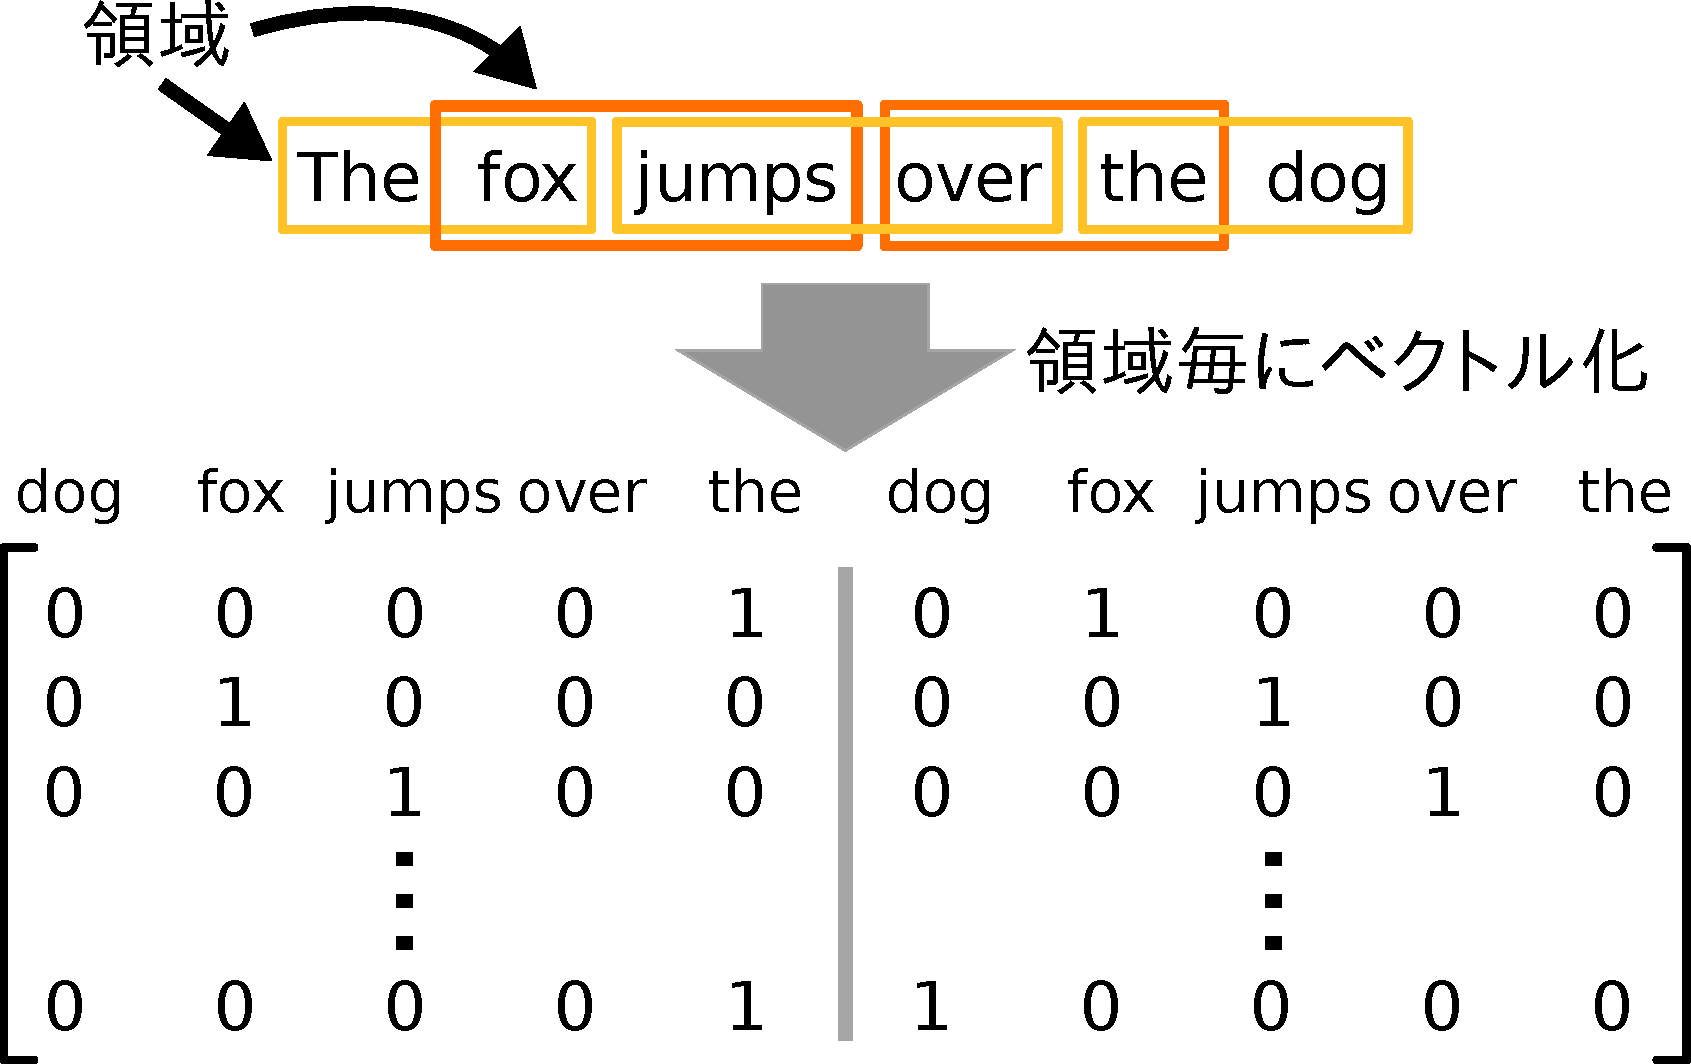
\includegraphics{fig/seq_cnn_text_feature.pdf}
  \caption{seq-CNNにおける文書の素性の構成}
  \label{fig:SeqCNNTextFeature}
\end{figure}
一方、bow-CNNにおける文書の素性は、各領域毎のベクトルが
その領域のBOWであるような行列である。
実験では、Bag Of n-gramsによる文書の素性とSVMによる手法を含む他の手法に比べ、
seq-CNNとbow-CNNの畳み込み\nn の部分を並列に全結合\nn に結合したモデルが
低い誤り率を示した。

Duyuらの手法は、単語ベクトルに対する畳み込み\nn に対し
ユーザ及び商品を表すパラメータを追加し拡張した手法である。
このモデルはUser Product Neural Network (UPNN)と呼ばれる。
Duyuらはレビューのデータセットに対して、
ユーザが付与するレーティングの一貫性、
商品が付与されるレーティングの一貫性、
ユーザの単語の使用に関する一貫性、
商品のレビュー文書に使用される単語の一貫性が
それぞれ成立することを検証した。
そこで、UPNNではこの4つの一貫性を表すパラメータがモデルに追加されている。
ユーザの単語の使用に関する一貫性、
商品のレビュー文書に使用される単語の一貫性はそれぞれ行列$U_k$と$P_j$で
表される。
ここで、$k$はユーザ、$j$は商品を表す。
これらの行列は畳み込みニューラルネットワークの入力となる各単語ベクトルを
式\ref{eq:UPNNProjectWord}のように写像する。
\begin{gather} \label{eq:UPNNProjectWord}
  w' = \left[ \begin{array}{c} U_k \\ P_j \end{array} \right] w
\end{gather}
ここで、$w$は単語ベクトル、$w'$は写像された単語ベクトルである。
次に、ユーザが付与するレーティングの一貫性、
商品が付与されるレーティングの一貫性はそれぞれベクトル$u_k$と$p_j$で
表される。
これらは畳み込み\nn の出力値と共に全結合\nn によって分類に利用される。
以上の行列$U_k$と$P_j$、及び、ベクトル$u_k$と$p_j$により、
検証された4つの一貫性を考慮したレーティング予測を行うことができる。
実験では、UPNNが他の手法より高い正答率を示している。
また、UPNNと各一貫性を表現するパラメータをUPNNから取り除いたモデルを
比較することで、各パラメータが確かに正答率の向上に有効であることが
示されている。

以上の手法は、レビューの特徴を各観点から上手く考慮している一方で、
1つのカテゴリにおける多値または二値分類を対象としている。
よって、多カテゴリのレーティング予測において、これらの手法をカテゴリ毎に
適用しただけではカテゴリ間の関係を考慮することができない。


\subsection{形態素解析}

形態素解析とは、文等の文字列を形態素に分割する処理である\cite{hozumi06}。
ここで、形態素とは意味を持った言語の最小単位である。
日本語における形態素解析は、単語分割とその語形変化の解析に相当する。
以降、日本語の文字列を形態素解析する場合の単語分割について述べる。
単語分割の手法として、最長一致法と
%分割数最小法、
bi-gramマルコフモデルによるものについて説明する。

最長一致法では、解析すべき文字列を順に読み進めながら
解析結果となる単語を決定していく。
まず、文字列の現在の位置からの部分文字列が辞書内の単語と一致するか検査する。
次に、一致した単語の内最も文字数の多いものを解析された単語として記録する。
最後に、その単語の文字数だけ文字列を読み進め、
再び現在の位置から始まる部分文字列に一致する単語を辞書で検索する。
これを繰り返していくことによって、文字列の終端まで形態素解析を行う。

これに対して、bi-gramマルコフモデルによる手法では単語のbi-gram確率を考え、
この積が文字列全体で最大となるように文字列を単語に分割する。
以下に最も適切な単語列$\hat{W}$を求める式を示す。
\begin{gather}
  \hat{W} = \text{argmax}_{W} P(W), \\
  P(W) = \sum^{n}_{i = 1} P(w_i | w_{i - 1}), \nonumber \\
  W = w_1, w_2, ... , w_n \nonumber
\end{gather}
ここで、$W$は元の文字列から分割された単語列であり、
$P(W)$はその単語列の同時確率である。
$w_i$は単語、$P(w_i | w_{i - 1})$は単語$w_i$と単語$w_{i - 1}$の
bi-gram確率である。


\subsection{Adam}

Adam\cite{diederik15}は確率的最適化のためのパラメータ更新のアルゴリズムである。
実験によって、Adamがニューラルネットワークに適用できること、及び、
パラメータをSGDやAdaGrad\cite{john12}より速く収束させることが
確かめられている。
式\ref{eq:AdamUpdate}にAdamによる目的関数$L$のパラメータ$\vc{w}$の
更新式を示す。
式\ref{eq:AdamUpdate}は、実際にはDiederikら\cite{diederik15}によって
示されている逐次的なアルゴリズムによって効率良く実装できる。
\begin{gather} \label{eq:AdamUpdate}
  \vc{w}_t = \vc{w}_{t - 1}
                 - \alpha \frac{\vc{m}_t}
                               {\sqrt{\vc{v}_t} + \epsilon}, \\
  \vc{m}_t = \frac{1 - \beta_1}{1 - {\beta_1}^t}
                 \sum^t_{i = 1} {\beta_1}^{t - i} \vc{g}_i, \nonumber \\
  \vc{v}_t = \frac{1 - \beta_2}{1 - {\beta_2}^t}
                 \sum^t_{i = 1} {\beta_2}^{t - i} {\vc{g}_i}^2, \nonumber \\
  \vc{g}_i = \frac{\partial L_i}{\partial \vc{w}_i} \nonumber
\end{gather}
ここで、$\vc{w}_t$は更新回数$t$におけるパラメータ$\vc{w}$を表す。
$\vc{m}_t$と$\vc{v}_t$は更新回数$t$における
パラメータ$\vc{w}$の一次・二次モーメントである。
$\alpha$と$\beta_1$、$\beta_2$、$\epsilon$はAdamのパラメータである。
$\vc{g}_t$は更新回数$t$におけるパラメータ$\vc{w}$の勾配である。

Adamの特徴として、$\alpha \frac{\vc{m}_t}{\sqrt{\vc{v}_t}}
\underset{\approx}{<} \alpha$である。
$\alpha \frac{\vc{m}_t}{\sqrt{\vc{v}_t}}$は全ての$t$について
$g_t$を定数倍しても変化しない。
よって、更新幅の大まかな上限を実際に計算される勾配$g_t$に依らず
$\alpha$のみによって決定することができる。
また、Diederikら\cite{diederik15}は
$\frac{\vc{m}_t}{\sqrt{\vc{v}_t}}$をsignal-to-noise ratio (SNR)と
呼んでいる。
SNRの分子$\vc{m}_t$は、更新回数$t$までの更新幅が小さい、あるいは、
勾配の向きがよく変わっているとき小さくなる。
よって、パラメータが最適解や局所解、鞍点付近にあるときは更新幅が小さくなり、
それ以外のとき大きくなる。
%SNRの分母$\vc{v}_t$は、更新回数$t$までの更新幅が大きいとき大きくなる。
%よって、パラメータが更新回数$t$までに大きく更新されているとき
%更新幅は小さくなる。
